% Generated by figures/teaser_drawio_to_tikz.py from paper/figs/fig_teaser.drawio -- do not edit by hand.
% Include with \resizebox{\textwidth}{!}{% Generated by figures/teaser_drawio_to_tikz.py from paper/figs/fig_teaser.drawio -- do not edit by hand.
% Include with \resizebox{\textwidth}{!}{% Generated by figures/teaser_drawio_to_tikz.py from paper/figs/fig_teaser.drawio -- do not edit by hand.
% Include with \resizebox{\textwidth}{!}{% Generated by figures/teaser_drawio_to_tikz.py from paper/figs/fig_teaser.drawio -- do not edit by hand.
% Include with \resizebox{\textwidth}{!}{\input{Figures/fig_teaser_tikz}} (needs \usetikzlibrary{arrows.meta}).
\definecolor{rgbhex1d221c}{HTML}{1D221C}
\definecolor{rgbhex2a9d8f}{HTML}{2A9D8F}
\definecolor{rgbhex2b3a67}{HTML}{2B3A67}
\definecolor{rgbhex30638e}{HTML}{30638E}
\definecolor{rgbhex5f685c}{HTML}{5F685C}
\definecolor{rgbhexb8860b}{HTML}{B8860B}
\definecolor{rgbhexc0392b}{HTML}{C0392B}
\definecolor{rgbhexeef1f7}{HTML}{EEF1F7}
\begin{tikzpicture}[x=0.005in, y=-0.005in]
\useasboundingbox (0,0) rectangle (1410,630);
\draw[draw={rgbhex2b3a67}, line width=1.30pt, rounded corners=8.6pt, fill={rgbhexeef1f7}] (560.0,138.0) rectangle (736.0,562.0);
\node[anchor=north west, inner sep=0] at (60.0,138.0) {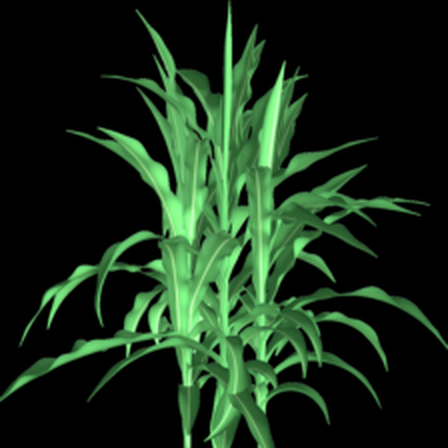
\includegraphics[width=0.7400in, height=0.7400in]{Figures/teaser/s_rgb.png}};
\node[anchor=north west, inner sep=0] at (218.0,138.0) {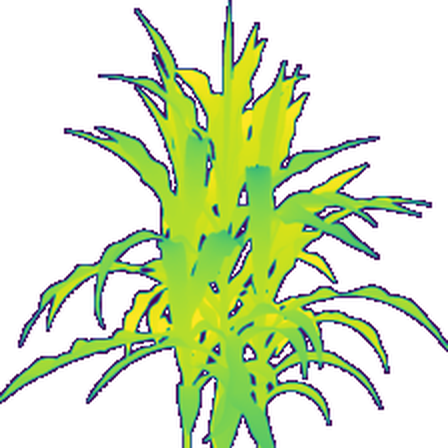
\includegraphics[width=0.7400in, height=0.7400in]{Figures/teaser/s_depth.png}};
\node[anchor=north west, inner sep=0] at (370.0,132.0) {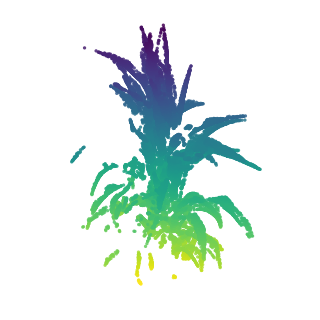
\includegraphics[width=0.8000in, height=0.8000in]{Figures/teaser/s_pc.png}};
\node[anchor=north west, inner sep=0] at (1074.0,132.0) {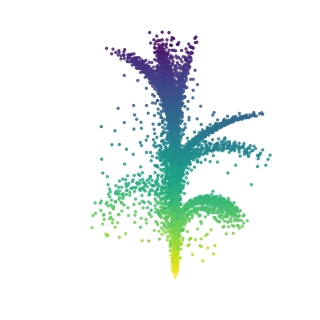
\includegraphics[width=0.8000in, height=0.8000in]{Figures/teaser/s_gen.png}};
\node[anchor=north west, inner sep=0] at (60.0,414.0) {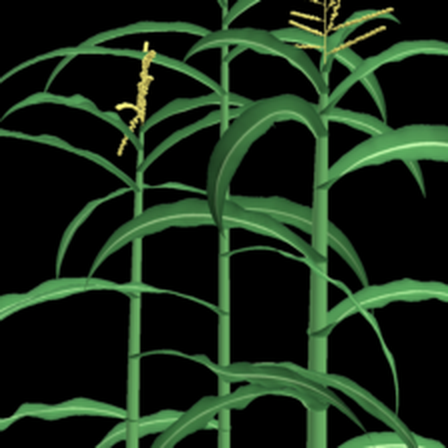
\includegraphics[width=0.7400in, height=0.7400in]{Figures/teaser/m_rgb.png}};
\node[anchor=north west, inner sep=0] at (218.0,414.0) {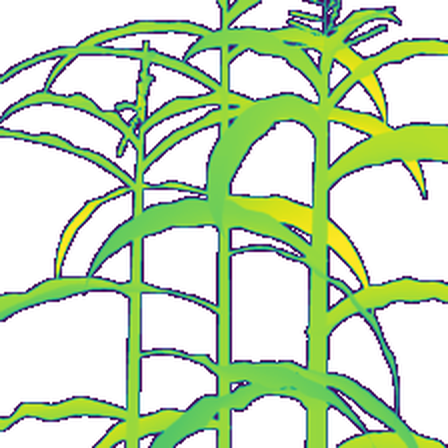
\includegraphics[width=0.7400in, height=0.7400in]{Figures/teaser/m_depth.png}};
\node[anchor=north west, inner sep=0] at (370.0,408.0) {
\includegraphics[width=0.8000in, height=0.8000in]{Figures/teaser/m_pc.png}};
\node[anchor=north west, inner sep=0] at (1074.0,408.0) {
\includegraphics[width=0.8000in, height=0.8000in]{Figures/teaser/m_gen.png}};
\draw[draw={rgbhexc0392b}, line width=1.01pt, rounded corners=5.8pt] (60.0,138.0) rectangle (208.0,286.0);
\draw[draw={rgbhexb8860b}, line width=1.01pt, rounded corners=5.8pt] (218.0,138.0) rectangle (366.0,286.0);
\draw[draw={rgbhex2a9d8f}, line width=1.01pt, rounded corners=5.8pt] (376.0,138.0) rectangle (524.0,286.0);
\draw[draw={rgbhex30638e}, line width=1.01pt, rounded corners=5.8pt] (784.0,138.0) rectangle (1048.0,286.0);
\draw[draw={rgbhex2a9d8f}, line width=1.01pt, rounded corners=5.8pt] (1080.0,138.0) rectangle (1228.0,286.0);
\draw[draw={rgbhex1d221c}, line width=0.61pt, rounded corners=5.8pt] (1240.0,138.0) rectangle (1406.0,286.0);
\draw[draw={rgbhexc0392b}, line width=1.01pt, rounded corners=5.8pt] (60.0,414.0) rectangle (208.0,562.0);
\draw[draw={rgbhexb8860b}, line width=1.01pt, rounded corners=5.8pt] (218.0,414.0) rectangle (366.0,562.0);
\draw[draw={rgbhex2a9d8f}, line width=1.01pt, rounded corners=5.8pt] (376.0,414.0) rectangle (524.0,562.0);
\draw[draw={rgbhex30638e}, line width=1.01pt, rounded corners=5.8pt] (784.0,414.0) rectangle (1048.0,562.0);
\draw[draw={rgbhex2a9d8f}, line width=1.01pt, rounded corners=5.8pt] (1080.0,414.0) rectangle (1228.0,562.0);
\draw[draw={rgbhex1d221c}, line width=0.61pt, rounded corners=5.8pt] (1240.0,414.0) rectangle (1406.0,562.0);
\node[anchor=west, inner sep=0, align=left, text={rgbhex1d221c}, font={\fontsize{7.5}{9.4}\selectfont\sffamily\bfseries}] at (60.0,42.0) {A simulated crop row, as a rover sees it};
\node[anchor=center, inner sep=0, align=center, text={rgbhex1d221c}, font={\fontsize{7.5}{9.4}\selectfont\sffamily\bfseries}] at (648.0,42.0) {One model};
\node[anchor=west, inner sep=0, align=left, text={rgbhex1d221c}, font={\fontsize{7.5}{9.4}\selectfont\sffamily\bfseries}] at (784.0,42.0) {The center plant out, and what it gives};
\node[anchor=center, inner sep=0, align=center, text={rgbhexc0392b}, font={\fontsize{6.2}{7.7}\selectfont\sffamily\bfseries}] at (134.1,86.0) {Image};
\node[anchor=center, inner sep=0, align=center, text={rgbhexb8860b}, font={\fontsize{6.2}{7.7}\selectfont\sffamily\bfseries}] at (292.1,86.0) {Depth image};
\node[anchor=center, inner sep=0, align=center, text={rgbhex2a9d8f}, font={\fontsize{6.2}{7.7}\selectfont\sffamily\bfseries}] at (450.1,86.0) {Point cloud};
\node[anchor=center, inner sep=0, align=center, text={rgbhex30638e}, font={\fontsize{6.2}{7.7}\selectfont\sffamily\bfseries}] at (916.0,86.0) {Procedural parameters};
\node[anchor=center, inner sep=0, align=center, text={rgbhex2a9d8f}, font={\fontsize{6.2}{7.7}\selectfont\sffamily\bfseries}] at (1154.0,86.0) {Generated point cloud};
\node[anchor=center, inner sep=0, align=center, text={rgbhex1d221c}, font={\fontsize{6.2}{7.7}\selectfont\sffamily\bfseries}] at (1323.0,86.0) {Traits};
\node[anchor=center, inner sep=0, align=center, text={rgbhex2b3a67}, font={\fontsize{8.0}{10.0}\selectfont\sffamily\bfseries}] at (647.9,306.0) {CropCode};
\node[anchor=center, inner sep=0, align=center, text={rgbhex2b3a67}, font={\fontsize{5.0}{6.3}\selectfont\sffamily}] at (647.9,382.1) {one encoder for\\photographs, depth,\\clouds and recipes;\\pretrained on single\\plants, then\\fine-tuned on crop\\rows to write the\\center plant};
\node[anchor=center, inner sep=0, align=center, text={rgbhex1d221c}, font={\fontsize{7.0}{8.7}\selectfont\sffamily\bfseries}, rotate=90] at (26.0,211.9) {sorghum};
\draw[color={rgbhex1d221c}, line width=0.90pt, -{Triangle[length=3.2pt,width=2.6pt]}] (528.0,212.0) -- (556.0,212.0);
\node[anchor=north west, inner sep=0, align=left, text={rgbhex5f685c}, font={\fontsize{4.6}{5.8}\selectfont\sffamily}] at (60.0,300.0) {25 \% of the center plant is hidden by its neighbors};
\draw[color={rgbhex30638e}, line width=0.90pt, -{Triangle[length=3.2pt,width=2.6pt]}] (740.0,212.0) -- (780.0,212.0);
\node[anchor=north west, inner sep=0, align=left, text={rgbhex30638e}, font={\fontsize{4.4}{5.7}\selectfont\ttfamily}] at (792.0,146.0) {stem~1.12~m,~22~leaves\\leaf~start~~len~roll~branch~width\\~~1~~~0.19~0.27~~171~~~~~20~0.091\\~~2~~~0.22~0.40~~171~~~~~21~0.093\\~~3~~~0.26~0.54~~314~~~~~21~0.093\\~~4~~~0.30~0.62~~176~~~~~21~0.093\\~~5~~~0.34~0.66~~320~~~~~21~0.100\\~~~~~\dots{}~17~more~leaves};
\draw[color={rgbhex2a9d8f}, line width=0.90pt, -{Triangle[length=3.2pt,width=2.6pt]}] (1052.0,212.0) -- (1076.0,212.0);
\node[anchor=north, inner sep=0, align=center, text={rgbhex5f685c}, font={\fontsize{4.6}{5.8}\selectfont\sffamily}] at (1154.0,300.0) {Chamfer 19.6e-4 m\textsuperscript{2} vs the true plant};
\node[anchor=north west, inner sep=0, align=left, text={rgbhex1d221c}, font={\fontsize{4.4}{5.3}\selectfont\sffamily}] at (1248.0,146.0) {height\\~~1.12m (true 1.10m)\\leaves\\~~22 (true 21)\\leaf length\\~~0.75m (true 0.75m)\\leaf width\\~~9.9cm (true 10.4cm)};
\node[anchor=center, inner sep=0, align=center, text={rgbhex1d221c}, font={\fontsize{7.0}{8.7}\selectfont\sffamily\bfseries}, rotate=90] at (26.0,488.0) {maize};
\draw[color={rgbhex1d221c}, line width=0.90pt, -{Triangle[length=3.2pt,width=2.6pt]}] (528.0,488.0) -- (556.0,488.0);
\node[anchor=north west, inner sep=0, align=left, text={rgbhex5f685c}, font={\fontsize{4.6}{5.8}\selectfont\sffamily}] at (60.0,576.0) {22 \% of the center plant is hidden by its neighbors};
\draw[color={rgbhex30638e}, line width=0.90pt, -{Triangle[length=3.2pt,width=2.6pt]}] (740.0,488.0) -- (780.0,488.0);
\node[anchor=north west, inner sep=0, align=left, text={rgbhex30638e}, font={\fontsize{4.4}{5.7}\selectfont\ttfamily}] at (792.0,422.0) {height~1.07~m,~13~leaves\\leaf~~dist~~len~~~wid~angle~droop\\~~1~~0.092~0.34~0.062~~~~-7~~~-92\\~~2~~0.091~0.36~0.063~~~~-2~~~-91\\~~3~~0.093~0.41~0.068~~~~-4~~~-93\\~~4~~0.092~0.44~0.064~~~~13~~~-94\\~~5~~0.093~0.44~0.063~~~~-3~~~-95\\~~~~~\dots{}~8~more~leaves};
\draw[color={rgbhex2a9d8f}, line width=0.90pt, -{Triangle[length=3.2pt,width=2.6pt]}] (1052.0,488.0) -- (1076.0,488.0);
\node[anchor=north, inner sep=0, align=center, text={rgbhex5f685c}, font={\fontsize{4.6}{5.8}\selectfont\sffamily}] at (1154.0,576.0) {Chamfer 2.6e-4 m\textsuperscript{2} vs the true plant};
\node[anchor=north west, inner sep=0, align=left, text={rgbhex1d221c}, font={\fontsize{4.4}{5.3}\selectfont\sffamily}] at (1248.0,422.0) {height\\~~1.07m (true 1.06m)\\leaves\\~~13 (true 13)\\leaf length\\~~0.36m (true 0.37m)\\leaf angle\\~~13$^\circ$ (true 13$^\circ$)};
\node[anchor=west, inner sep=0, align=left, text={rgbhex5f685c}, font={\fontsize{4.6}{5.8}\selectfont\sffamily\itshape}] at (60.0,606.0) {Held-out test rows, seen broadside by the rover camera; nothing marks the center plant. The true plant is shown for comparison only.};
\end{tikzpicture}
} (needs \usetikzlibrary{arrows.meta}).
\definecolor{rgbhex1d221c}{HTML}{1D221C}
\definecolor{rgbhex2a9d8f}{HTML}{2A9D8F}
\definecolor{rgbhex2b3a67}{HTML}{2B3A67}
\definecolor{rgbhex30638e}{HTML}{30638E}
\definecolor{rgbhex5f685c}{HTML}{5F685C}
\definecolor{rgbhexb8860b}{HTML}{B8860B}
\definecolor{rgbhexc0392b}{HTML}{C0392B}
\definecolor{rgbhexeef1f7}{HTML}{EEF1F7}
\begin{tikzpicture}[x=0.005in, y=-0.005in]
\useasboundingbox (0,0) rectangle (1410,630);
\draw[draw={rgbhex2b3a67}, line width=1.30pt, rounded corners=8.6pt, fill={rgbhexeef1f7}] (560.0,138.0) rectangle (736.0,562.0);
\node[anchor=north west, inner sep=0] at (60.0,138.0) {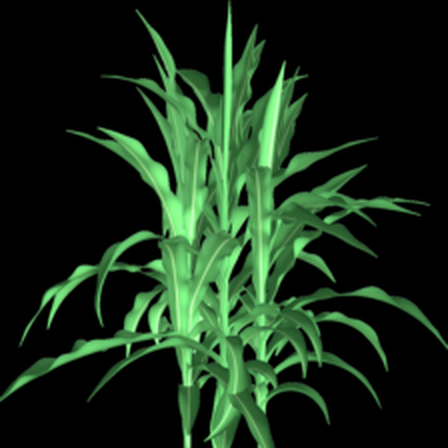
\includegraphics[width=0.7400in, height=0.7400in]{Figures/teaser/s_rgb.png}};
\node[anchor=north west, inner sep=0] at (218.0,138.0) {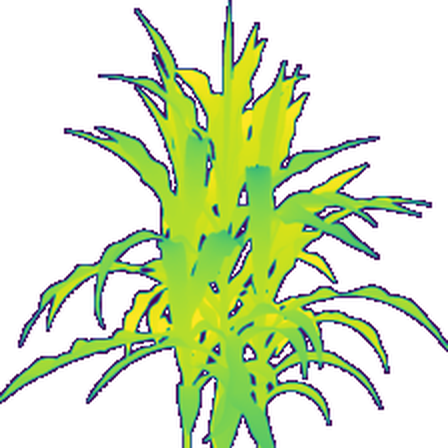
\includegraphics[width=0.7400in, height=0.7400in]{Figures/teaser/s_depth.png}};
\node[anchor=north west, inner sep=0] at (370.0,132.0) {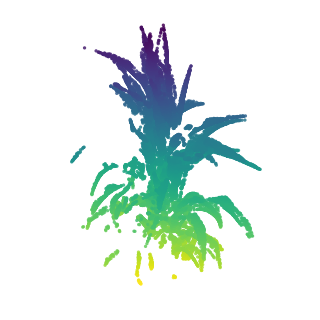
\includegraphics[width=0.8000in, height=0.8000in]{Figures/teaser/s_pc.png}};
\node[anchor=north west, inner sep=0] at (1074.0,132.0) {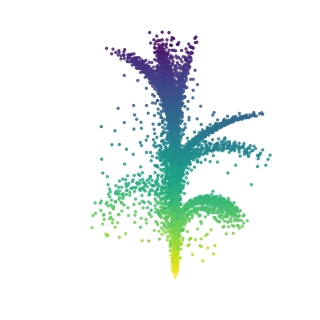
\includegraphics[width=0.8000in, height=0.8000in]{Figures/teaser/s_gen.png}};
\node[anchor=north west, inner sep=0] at (60.0,414.0) {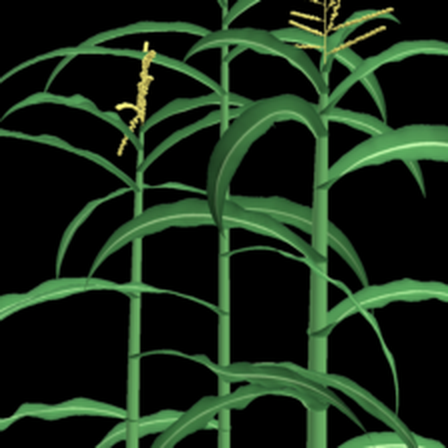
\includegraphics[width=0.7400in, height=0.7400in]{Figures/teaser/m_rgb.png}};
\node[anchor=north west, inner sep=0] at (218.0,414.0) {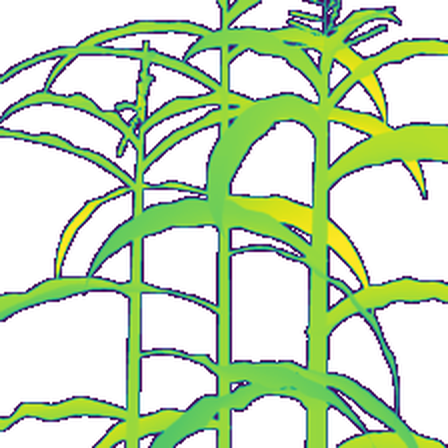
\includegraphics[width=0.7400in, height=0.7400in]{Figures/teaser/m_depth.png}};
\node[anchor=north west, inner sep=0] at (370.0,408.0) {
\includegraphics[width=0.8000in, height=0.8000in]{Figures/teaser/m_pc.png}};
\node[anchor=north west, inner sep=0] at (1074.0,408.0) {
\includegraphics[width=0.8000in, height=0.8000in]{Figures/teaser/m_gen.png}};
\draw[draw={rgbhexc0392b}, line width=1.01pt, rounded corners=5.8pt] (60.0,138.0) rectangle (208.0,286.0);
\draw[draw={rgbhexb8860b}, line width=1.01pt, rounded corners=5.8pt] (218.0,138.0) rectangle (366.0,286.0);
\draw[draw={rgbhex2a9d8f}, line width=1.01pt, rounded corners=5.8pt] (376.0,138.0) rectangle (524.0,286.0);
\draw[draw={rgbhex30638e}, line width=1.01pt, rounded corners=5.8pt] (784.0,138.0) rectangle (1048.0,286.0);
\draw[draw={rgbhex2a9d8f}, line width=1.01pt, rounded corners=5.8pt] (1080.0,138.0) rectangle (1228.0,286.0);
\draw[draw={rgbhex1d221c}, line width=0.61pt, rounded corners=5.8pt] (1240.0,138.0) rectangle (1406.0,286.0);
\draw[draw={rgbhexc0392b}, line width=1.01pt, rounded corners=5.8pt] (60.0,414.0) rectangle (208.0,562.0);
\draw[draw={rgbhexb8860b}, line width=1.01pt, rounded corners=5.8pt] (218.0,414.0) rectangle (366.0,562.0);
\draw[draw={rgbhex2a9d8f}, line width=1.01pt, rounded corners=5.8pt] (376.0,414.0) rectangle (524.0,562.0);
\draw[draw={rgbhex30638e}, line width=1.01pt, rounded corners=5.8pt] (784.0,414.0) rectangle (1048.0,562.0);
\draw[draw={rgbhex2a9d8f}, line width=1.01pt, rounded corners=5.8pt] (1080.0,414.0) rectangle (1228.0,562.0);
\draw[draw={rgbhex1d221c}, line width=0.61pt, rounded corners=5.8pt] (1240.0,414.0) rectangle (1406.0,562.0);
\node[anchor=west, inner sep=0, align=left, text={rgbhex1d221c}, font={\fontsize{7.5}{9.4}\selectfont\sffamily\bfseries}] at (60.0,42.0) {A simulated crop row, as a rover sees it};
\node[anchor=center, inner sep=0, align=center, text={rgbhex1d221c}, font={\fontsize{7.5}{9.4}\selectfont\sffamily\bfseries}] at (648.0,42.0) {One model};
\node[anchor=west, inner sep=0, align=left, text={rgbhex1d221c}, font={\fontsize{7.5}{9.4}\selectfont\sffamily\bfseries}] at (784.0,42.0) {The center plant out, and what it gives};
\node[anchor=center, inner sep=0, align=center, text={rgbhexc0392b}, font={\fontsize{6.2}{7.7}\selectfont\sffamily\bfseries}] at (134.1,86.0) {Image};
\node[anchor=center, inner sep=0, align=center, text={rgbhexb8860b}, font={\fontsize{6.2}{7.7}\selectfont\sffamily\bfseries}] at (292.1,86.0) {Depth image};
\node[anchor=center, inner sep=0, align=center, text={rgbhex2a9d8f}, font={\fontsize{6.2}{7.7}\selectfont\sffamily\bfseries}] at (450.1,86.0) {Point cloud};
\node[anchor=center, inner sep=0, align=center, text={rgbhex30638e}, font={\fontsize{6.2}{7.7}\selectfont\sffamily\bfseries}] at (916.0,86.0) {Procedural parameters};
\node[anchor=center, inner sep=0, align=center, text={rgbhex2a9d8f}, font={\fontsize{6.2}{7.7}\selectfont\sffamily\bfseries}] at (1154.0,86.0) {Generated point cloud};
\node[anchor=center, inner sep=0, align=center, text={rgbhex1d221c}, font={\fontsize{6.2}{7.7}\selectfont\sffamily\bfseries}] at (1323.0,86.0) {Traits};
\node[anchor=center, inner sep=0, align=center, text={rgbhex2b3a67}, font={\fontsize{8.0}{10.0}\selectfont\sffamily\bfseries}] at (647.9,306.0) {CropCode};
\node[anchor=center, inner sep=0, align=center, text={rgbhex2b3a67}, font={\fontsize{5.0}{6.3}\selectfont\sffamily}] at (647.9,382.1) {one encoder for\\photographs, depth,\\clouds and recipes;\\pretrained on single\\plants, then\\fine-tuned on crop\\rows to write the\\center plant};
\node[anchor=center, inner sep=0, align=center, text={rgbhex1d221c}, font={\fontsize{7.0}{8.7}\selectfont\sffamily\bfseries}, rotate=90] at (26.0,211.9) {sorghum};
\draw[color={rgbhex1d221c}, line width=0.90pt, -{Triangle[length=3.2pt,width=2.6pt]}] (528.0,212.0) -- (556.0,212.0);
\node[anchor=north west, inner sep=0, align=left, text={rgbhex5f685c}, font={\fontsize{4.6}{5.8}\selectfont\sffamily}] at (60.0,300.0) {25 \% of the center plant is hidden by its neighbors};
\draw[color={rgbhex30638e}, line width=0.90pt, -{Triangle[length=3.2pt,width=2.6pt]}] (740.0,212.0) -- (780.0,212.0);
\node[anchor=north west, inner sep=0, align=left, text={rgbhex30638e}, font={\fontsize{4.4}{5.7}\selectfont\ttfamily}] at (792.0,146.0) {stem~1.12~m,~22~leaves\\leaf~start~~len~roll~branch~width\\~~1~~~0.19~0.27~~171~~~~~20~0.091\\~~2~~~0.22~0.40~~171~~~~~21~0.093\\~~3~~~0.26~0.54~~314~~~~~21~0.093\\~~4~~~0.30~0.62~~176~~~~~21~0.093\\~~5~~~0.34~0.66~~320~~~~~21~0.100\\~~~~~\dots{}~17~more~leaves};
\draw[color={rgbhex2a9d8f}, line width=0.90pt, -{Triangle[length=3.2pt,width=2.6pt]}] (1052.0,212.0) -- (1076.0,212.0);
\node[anchor=north, inner sep=0, align=center, text={rgbhex5f685c}, font={\fontsize{4.6}{5.8}\selectfont\sffamily}] at (1154.0,300.0) {Chamfer 19.6e-4 m\textsuperscript{2} vs the true plant};
\node[anchor=north west, inner sep=0, align=left, text={rgbhex1d221c}, font={\fontsize{4.4}{5.3}\selectfont\sffamily}] at (1248.0,146.0) {height\\~~1.12m (true 1.10m)\\leaves\\~~22 (true 21)\\leaf length\\~~0.75m (true 0.75m)\\leaf width\\~~9.9cm (true 10.4cm)};
\node[anchor=center, inner sep=0, align=center, text={rgbhex1d221c}, font={\fontsize{7.0}{8.7}\selectfont\sffamily\bfseries}, rotate=90] at (26.0,488.0) {maize};
\draw[color={rgbhex1d221c}, line width=0.90pt, -{Triangle[length=3.2pt,width=2.6pt]}] (528.0,488.0) -- (556.0,488.0);
\node[anchor=north west, inner sep=0, align=left, text={rgbhex5f685c}, font={\fontsize{4.6}{5.8}\selectfont\sffamily}] at (60.0,576.0) {22 \% of the center plant is hidden by its neighbors};
\draw[color={rgbhex30638e}, line width=0.90pt, -{Triangle[length=3.2pt,width=2.6pt]}] (740.0,488.0) -- (780.0,488.0);
\node[anchor=north west, inner sep=0, align=left, text={rgbhex30638e}, font={\fontsize{4.4}{5.7}\selectfont\ttfamily}] at (792.0,422.0) {height~1.07~m,~13~leaves\\leaf~~dist~~len~~~wid~angle~droop\\~~1~~0.092~0.34~0.062~~~~-7~~~-92\\~~2~~0.091~0.36~0.063~~~~-2~~~-91\\~~3~~0.093~0.41~0.068~~~~-4~~~-93\\~~4~~0.092~0.44~0.064~~~~13~~~-94\\~~5~~0.093~0.44~0.063~~~~-3~~~-95\\~~~~~\dots{}~8~more~leaves};
\draw[color={rgbhex2a9d8f}, line width=0.90pt, -{Triangle[length=3.2pt,width=2.6pt]}] (1052.0,488.0) -- (1076.0,488.0);
\node[anchor=north, inner sep=0, align=center, text={rgbhex5f685c}, font={\fontsize{4.6}{5.8}\selectfont\sffamily}] at (1154.0,576.0) {Chamfer 2.6e-4 m\textsuperscript{2} vs the true plant};
\node[anchor=north west, inner sep=0, align=left, text={rgbhex1d221c}, font={\fontsize{4.4}{5.3}\selectfont\sffamily}] at (1248.0,422.0) {height\\~~1.07m (true 1.06m)\\leaves\\~~13 (true 13)\\leaf length\\~~0.36m (true 0.37m)\\leaf angle\\~~13$^\circ$ (true 13$^\circ$)};
\node[anchor=west, inner sep=0, align=left, text={rgbhex5f685c}, font={\fontsize{4.6}{5.8}\selectfont\sffamily\itshape}] at (60.0,606.0) {Held-out test rows, seen broadside by the rover camera; nothing marks the center plant. The true plant is shown for comparison only.};
\end{tikzpicture}
} (needs \usetikzlibrary{arrows.meta}).
\definecolor{rgbhex1d221c}{HTML}{1D221C}
\definecolor{rgbhex2a9d8f}{HTML}{2A9D8F}
\definecolor{rgbhex2b3a67}{HTML}{2B3A67}
\definecolor{rgbhex30638e}{HTML}{30638E}
\definecolor{rgbhex5f685c}{HTML}{5F685C}
\definecolor{rgbhexb8860b}{HTML}{B8860B}
\definecolor{rgbhexc0392b}{HTML}{C0392B}
\definecolor{rgbhexeef1f7}{HTML}{EEF1F7}
\begin{tikzpicture}[x=0.005in, y=-0.005in]
\useasboundingbox (0,0) rectangle (1410,630);
\draw[draw={rgbhex2b3a67}, line width=1.30pt, rounded corners=8.6pt, fill={rgbhexeef1f7}] (560.0,138.0) rectangle (736.0,562.0);
\node[anchor=north west, inner sep=0] at (60.0,138.0) {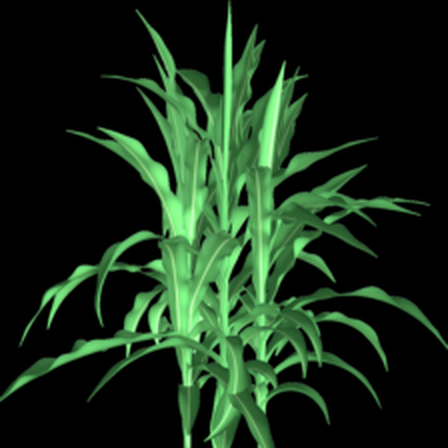
\includegraphics[width=0.7400in, height=0.7400in]{Figures/teaser/s_rgb.png}};
\node[anchor=north west, inner sep=0] at (218.0,138.0) {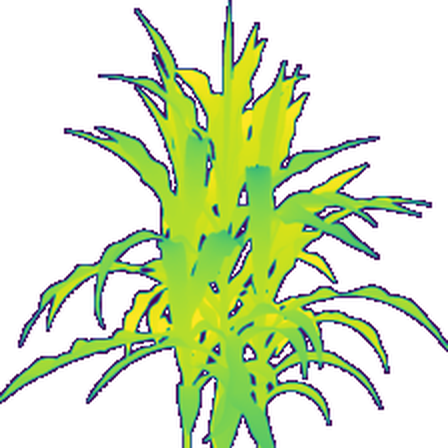
\includegraphics[width=0.7400in, height=0.7400in]{Figures/teaser/s_depth.png}};
\node[anchor=north west, inner sep=0] at (370.0,132.0) {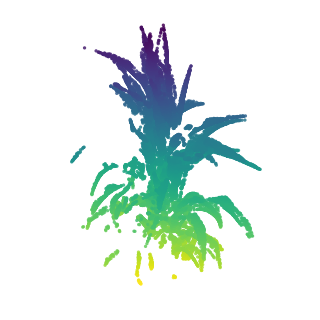
\includegraphics[width=0.8000in, height=0.8000in]{Figures/teaser/s_pc.png}};
\node[anchor=north west, inner sep=0] at (1074.0,132.0) {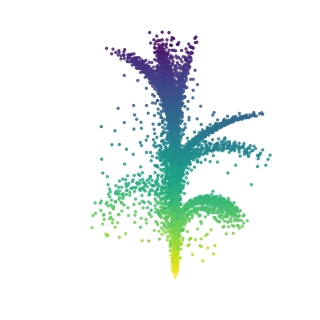
\includegraphics[width=0.8000in, height=0.8000in]{Figures/teaser/s_gen.png}};
\node[anchor=north west, inner sep=0] at (60.0,414.0) {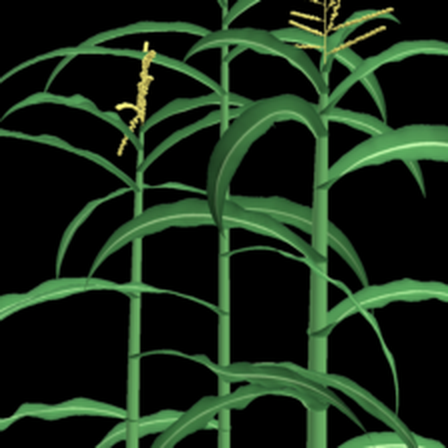
\includegraphics[width=0.7400in, height=0.7400in]{Figures/teaser/m_rgb.png}};
\node[anchor=north west, inner sep=0] at (218.0,414.0) {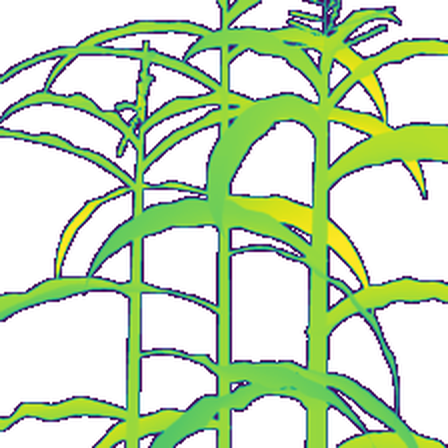
\includegraphics[width=0.7400in, height=0.7400in]{Figures/teaser/m_depth.png}};
\node[anchor=north west, inner sep=0] at (370.0,408.0) {
\includegraphics[width=0.8000in, height=0.8000in]{Figures/teaser/m_pc.png}};
\node[anchor=north west, inner sep=0] at (1074.0,408.0) {
\includegraphics[width=0.8000in, height=0.8000in]{Figures/teaser/m_gen.png}};
\draw[draw={rgbhexc0392b}, line width=1.01pt, rounded corners=5.8pt] (60.0,138.0) rectangle (208.0,286.0);
\draw[draw={rgbhexb8860b}, line width=1.01pt, rounded corners=5.8pt] (218.0,138.0) rectangle (366.0,286.0);
\draw[draw={rgbhex2a9d8f}, line width=1.01pt, rounded corners=5.8pt] (376.0,138.0) rectangle (524.0,286.0);
\draw[draw={rgbhex30638e}, line width=1.01pt, rounded corners=5.8pt] (784.0,138.0) rectangle (1048.0,286.0);
\draw[draw={rgbhex2a9d8f}, line width=1.01pt, rounded corners=5.8pt] (1080.0,138.0) rectangle (1228.0,286.0);
\draw[draw={rgbhex1d221c}, line width=0.61pt, rounded corners=5.8pt] (1240.0,138.0) rectangle (1406.0,286.0);
\draw[draw={rgbhexc0392b}, line width=1.01pt, rounded corners=5.8pt] (60.0,414.0) rectangle (208.0,562.0);
\draw[draw={rgbhexb8860b}, line width=1.01pt, rounded corners=5.8pt] (218.0,414.0) rectangle (366.0,562.0);
\draw[draw={rgbhex2a9d8f}, line width=1.01pt, rounded corners=5.8pt] (376.0,414.0) rectangle (524.0,562.0);
\draw[draw={rgbhex30638e}, line width=1.01pt, rounded corners=5.8pt] (784.0,414.0) rectangle (1048.0,562.0);
\draw[draw={rgbhex2a9d8f}, line width=1.01pt, rounded corners=5.8pt] (1080.0,414.0) rectangle (1228.0,562.0);
\draw[draw={rgbhex1d221c}, line width=0.61pt, rounded corners=5.8pt] (1240.0,414.0) rectangle (1406.0,562.0);
\node[anchor=west, inner sep=0, align=left, text={rgbhex1d221c}, font={\fontsize{7.5}{9.4}\selectfont\sffamily\bfseries}] at (60.0,42.0) {A simulated crop row, as a rover sees it};
\node[anchor=center, inner sep=0, align=center, text={rgbhex1d221c}, font={\fontsize{7.5}{9.4}\selectfont\sffamily\bfseries}] at (648.0,42.0) {One model};
\node[anchor=west, inner sep=0, align=left, text={rgbhex1d221c}, font={\fontsize{7.5}{9.4}\selectfont\sffamily\bfseries}] at (784.0,42.0) {The center plant out, and what it gives};
\node[anchor=center, inner sep=0, align=center, text={rgbhexc0392b}, font={\fontsize{6.2}{7.7}\selectfont\sffamily\bfseries}] at (134.1,86.0) {Image};
\node[anchor=center, inner sep=0, align=center, text={rgbhexb8860b}, font={\fontsize{6.2}{7.7}\selectfont\sffamily\bfseries}] at (292.1,86.0) {Depth image};
\node[anchor=center, inner sep=0, align=center, text={rgbhex2a9d8f}, font={\fontsize{6.2}{7.7}\selectfont\sffamily\bfseries}] at (450.1,86.0) {Point cloud};
\node[anchor=center, inner sep=0, align=center, text={rgbhex30638e}, font={\fontsize{6.2}{7.7}\selectfont\sffamily\bfseries}] at (916.0,86.0) {Procedural parameters};
\node[anchor=center, inner sep=0, align=center, text={rgbhex2a9d8f}, font={\fontsize{6.2}{7.7}\selectfont\sffamily\bfseries}] at (1154.0,86.0) {Generated point cloud};
\node[anchor=center, inner sep=0, align=center, text={rgbhex1d221c}, font={\fontsize{6.2}{7.7}\selectfont\sffamily\bfseries}] at (1323.0,86.0) {Traits};
\node[anchor=center, inner sep=0, align=center, text={rgbhex2b3a67}, font={\fontsize{8.0}{10.0}\selectfont\sffamily\bfseries}] at (647.9,306.0) {CropCode};
\node[anchor=center, inner sep=0, align=center, text={rgbhex2b3a67}, font={\fontsize{5.0}{6.3}\selectfont\sffamily}] at (647.9,382.1) {one encoder for\\photographs, depth,\\clouds and recipes;\\pretrained on single\\plants, then\\fine-tuned on crop\\rows to write the\\center plant};
\node[anchor=center, inner sep=0, align=center, text={rgbhex1d221c}, font={\fontsize{7.0}{8.7}\selectfont\sffamily\bfseries}, rotate=90] at (26.0,211.9) {sorghum};
\draw[color={rgbhex1d221c}, line width=0.90pt, -{Triangle[length=3.2pt,width=2.6pt]}] (528.0,212.0) -- (556.0,212.0);
\node[anchor=north west, inner sep=0, align=left, text={rgbhex5f685c}, font={\fontsize{4.6}{5.8}\selectfont\sffamily}] at (60.0,300.0) {25 \% of the center plant is hidden by its neighbors};
\draw[color={rgbhex30638e}, line width=0.90pt, -{Triangle[length=3.2pt,width=2.6pt]}] (740.0,212.0) -- (780.0,212.0);
\node[anchor=north west, inner sep=0, align=left, text={rgbhex30638e}, font={\fontsize{4.4}{5.7}\selectfont\ttfamily}] at (792.0,146.0) {stem~1.12~m,~22~leaves\\leaf~start~~len~roll~branch~width\\~~1~~~0.19~0.27~~171~~~~~20~0.091\\~~2~~~0.22~0.40~~171~~~~~21~0.093\\~~3~~~0.26~0.54~~314~~~~~21~0.093\\~~4~~~0.30~0.62~~176~~~~~21~0.093\\~~5~~~0.34~0.66~~320~~~~~21~0.100\\~~~~~\dots{}~17~more~leaves};
\draw[color={rgbhex2a9d8f}, line width=0.90pt, -{Triangle[length=3.2pt,width=2.6pt]}] (1052.0,212.0) -- (1076.0,212.0);
\node[anchor=north, inner sep=0, align=center, text={rgbhex5f685c}, font={\fontsize{4.6}{5.8}\selectfont\sffamily}] at (1154.0,300.0) {Chamfer 19.6e-4 m\textsuperscript{2} vs the true plant};
\node[anchor=north west, inner sep=0, align=left, text={rgbhex1d221c}, font={\fontsize{4.4}{5.3}\selectfont\sffamily}] at (1248.0,146.0) {height\\~~1.12m (true 1.10m)\\leaves\\~~22 (true 21)\\leaf length\\~~0.75m (true 0.75m)\\leaf width\\~~9.9cm (true 10.4cm)};
\node[anchor=center, inner sep=0, align=center, text={rgbhex1d221c}, font={\fontsize{7.0}{8.7}\selectfont\sffamily\bfseries}, rotate=90] at (26.0,488.0) {maize};
\draw[color={rgbhex1d221c}, line width=0.90pt, -{Triangle[length=3.2pt,width=2.6pt]}] (528.0,488.0) -- (556.0,488.0);
\node[anchor=north west, inner sep=0, align=left, text={rgbhex5f685c}, font={\fontsize{4.6}{5.8}\selectfont\sffamily}] at (60.0,576.0) {22 \% of the center plant is hidden by its neighbors};
\draw[color={rgbhex30638e}, line width=0.90pt, -{Triangle[length=3.2pt,width=2.6pt]}] (740.0,488.0) -- (780.0,488.0);
\node[anchor=north west, inner sep=0, align=left, text={rgbhex30638e}, font={\fontsize{4.4}{5.7}\selectfont\ttfamily}] at (792.0,422.0) {height~1.07~m,~13~leaves\\leaf~~dist~~len~~~wid~angle~droop\\~~1~~0.092~0.34~0.062~~~~-7~~~-92\\~~2~~0.091~0.36~0.063~~~~-2~~~-91\\~~3~~0.093~0.41~0.068~~~~-4~~~-93\\~~4~~0.092~0.44~0.064~~~~13~~~-94\\~~5~~0.093~0.44~0.063~~~~-3~~~-95\\~~~~~\dots{}~8~more~leaves};
\draw[color={rgbhex2a9d8f}, line width=0.90pt, -{Triangle[length=3.2pt,width=2.6pt]}] (1052.0,488.0) -- (1076.0,488.0);
\node[anchor=north, inner sep=0, align=center, text={rgbhex5f685c}, font={\fontsize{4.6}{5.8}\selectfont\sffamily}] at (1154.0,576.0) {Chamfer 2.6e-4 m\textsuperscript{2} vs the true plant};
\node[anchor=north west, inner sep=0, align=left, text={rgbhex1d221c}, font={\fontsize{4.4}{5.3}\selectfont\sffamily}] at (1248.0,422.0) {height\\~~1.07m (true 1.06m)\\leaves\\~~13 (true 13)\\leaf length\\~~0.36m (true 0.37m)\\leaf angle\\~~13$^\circ$ (true 13$^\circ$)};
\node[anchor=west, inner sep=0, align=left, text={rgbhex5f685c}, font={\fontsize{4.6}{5.8}\selectfont\sffamily\itshape}] at (60.0,606.0) {Held-out test rows, seen broadside by the rover camera; nothing marks the center plant. The true plant is shown for comparison only.};
\end{tikzpicture}
} (needs \usetikzlibrary{arrows.meta}).
\definecolor{rgbhex1d221c}{HTML}{1D221C}
\definecolor{rgbhex2a9d8f}{HTML}{2A9D8F}
\definecolor{rgbhex2b3a67}{HTML}{2B3A67}
\definecolor{rgbhex30638e}{HTML}{30638E}
\definecolor{rgbhex5f685c}{HTML}{5F685C}
\definecolor{rgbhexb8860b}{HTML}{B8860B}
\definecolor{rgbhexc0392b}{HTML}{C0392B}
\definecolor{rgbhexeef1f7}{HTML}{EEF1F7}
\begin{tikzpicture}[x=0.005in, y=-0.005in]
\useasboundingbox (0,0) rectangle (1410,630);
\draw[draw={rgbhex2b3a67}, line width=1.30pt, rounded corners=8.6pt, fill={rgbhexeef1f7}] (560.0,138.0) rectangle (736.0,562.0);
\node[anchor=north west, inner sep=0] at (60.0,138.0) {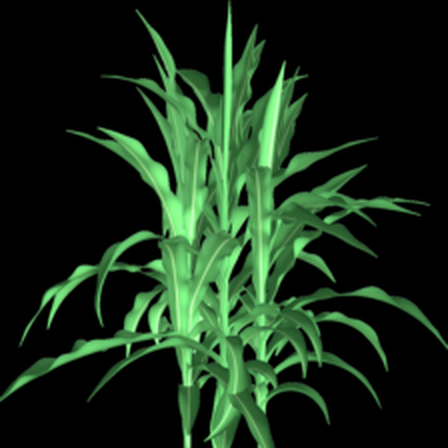
\includegraphics[width=0.7400in, height=0.7400in]{Figures/teaser/s_rgb.png}};
\node[anchor=north west, inner sep=0] at (218.0,138.0) {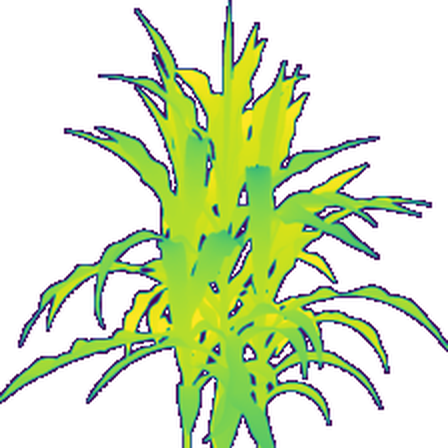
\includegraphics[width=0.7400in, height=0.7400in]{Figures/teaser/s_depth.png}};
\node[anchor=north west, inner sep=0] at (370.0,132.0) {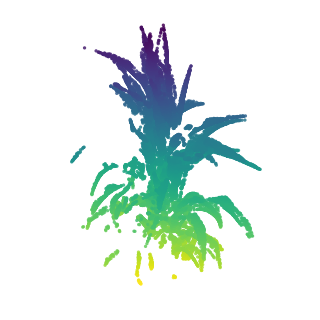
\includegraphics[width=0.8000in, height=0.8000in]{Figures/teaser/s_pc.png}};
\node[anchor=north west, inner sep=0] at (1074.0,132.0) {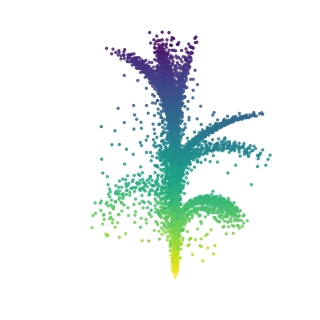
\includegraphics[width=0.8000in, height=0.8000in]{Figures/teaser/s_gen.png}};
\node[anchor=north west, inner sep=0] at (60.0,414.0) {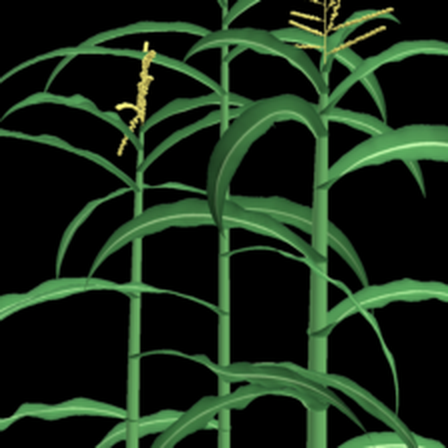
\includegraphics[width=0.7400in, height=0.7400in]{Figures/teaser/m_rgb.png}};
\node[anchor=north west, inner sep=0] at (218.0,414.0) {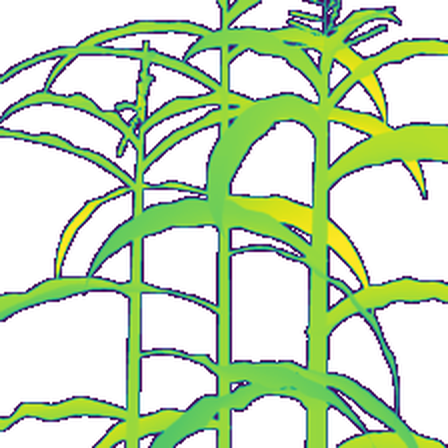
\includegraphics[width=0.7400in, height=0.7400in]{Figures/teaser/m_depth.png}};
\node[anchor=north west, inner sep=0] at (370.0,408.0) {
\includegraphics[width=0.8000in, height=0.8000in]{Figures/teaser/m_pc.png}};
\node[anchor=north west, inner sep=0] at (1074.0,408.0) {
\includegraphics[width=0.8000in, height=0.8000in]{Figures/teaser/m_gen.png}};
\draw[draw={rgbhexc0392b}, line width=1.01pt, rounded corners=5.8pt] (60.0,138.0) rectangle (208.0,286.0);
\draw[draw={rgbhexb8860b}, line width=1.01pt, rounded corners=5.8pt] (218.0,138.0) rectangle (366.0,286.0);
\draw[draw={rgbhex2a9d8f}, line width=1.01pt, rounded corners=5.8pt] (376.0,138.0) rectangle (524.0,286.0);
\draw[draw={rgbhex30638e}, line width=1.01pt, rounded corners=5.8pt] (784.0,138.0) rectangle (1048.0,286.0);
\draw[draw={rgbhex2a9d8f}, line width=1.01pt, rounded corners=5.8pt] (1080.0,138.0) rectangle (1228.0,286.0);
\draw[draw={rgbhex1d221c}, line width=0.61pt, rounded corners=5.8pt] (1240.0,138.0) rectangle (1406.0,286.0);
\draw[draw={rgbhexc0392b}, line width=1.01pt, rounded corners=5.8pt] (60.0,414.0) rectangle (208.0,562.0);
\draw[draw={rgbhexb8860b}, line width=1.01pt, rounded corners=5.8pt] (218.0,414.0) rectangle (366.0,562.0);
\draw[draw={rgbhex2a9d8f}, line width=1.01pt, rounded corners=5.8pt] (376.0,414.0) rectangle (524.0,562.0);
\draw[draw={rgbhex30638e}, line width=1.01pt, rounded corners=5.8pt] (784.0,414.0) rectangle (1048.0,562.0);
\draw[draw={rgbhex2a9d8f}, line width=1.01pt, rounded corners=5.8pt] (1080.0,414.0) rectangle (1228.0,562.0);
\draw[draw={rgbhex1d221c}, line width=0.61pt, rounded corners=5.8pt] (1240.0,414.0) rectangle (1406.0,562.0);
\node[anchor=west, inner sep=0, align=left, text={rgbhex1d221c}, font={\fontsize{7.5}{9.4}\selectfont\sffamily\bfseries}] at (60.0,42.0) {A simulated crop row, as a rover sees it};
\node[anchor=center, inner sep=0, align=center, text={rgbhex1d221c}, font={\fontsize{7.5}{9.4}\selectfont\sffamily\bfseries}] at (648.0,42.0) {One model};
\node[anchor=west, inner sep=0, align=left, text={rgbhex1d221c}, font={\fontsize{7.5}{9.4}\selectfont\sffamily\bfseries}] at (784.0,42.0) {The center plant out, and what it gives};
\node[anchor=center, inner sep=0, align=center, text={rgbhexc0392b}, font={\fontsize{6.2}{7.7}\selectfont\sffamily\bfseries}] at (134.1,86.0) {Image};
\node[anchor=center, inner sep=0, align=center, text={rgbhexb8860b}, font={\fontsize{6.2}{7.7}\selectfont\sffamily\bfseries}] at (292.1,86.0) {Depth image};
\node[anchor=center, inner sep=0, align=center, text={rgbhex2a9d8f}, font={\fontsize{6.2}{7.7}\selectfont\sffamily\bfseries}] at (450.1,86.0) {Point cloud};
\node[anchor=center, inner sep=0, align=center, text={rgbhex30638e}, font={\fontsize{6.2}{7.7}\selectfont\sffamily\bfseries}] at (916.0,86.0) {Procedural parameters};
\node[anchor=center, inner sep=0, align=center, text={rgbhex2a9d8f}, font={\fontsize{6.2}{7.7}\selectfont\sffamily\bfseries}] at (1154.0,86.0) {Generated point cloud};
\node[anchor=center, inner sep=0, align=center, text={rgbhex1d221c}, font={\fontsize{6.2}{7.7}\selectfont\sffamily\bfseries}] at (1323.0,86.0) {Traits};
\node[anchor=center, inner sep=0, align=center, text={rgbhex2b3a67}, font={\fontsize{8.0}{10.0}\selectfont\sffamily\bfseries}] at (647.9,306.0) {CropCode};
\node[anchor=center, inner sep=0, align=center, text={rgbhex2b3a67}, font={\fontsize{5.0}{6.3}\selectfont\sffamily}] at (647.9,382.1) {one encoder for\\photographs, depth,\\clouds and recipes;\\pretrained on single\\plants, then\\fine-tuned on crop\\rows to write the\\center plant};
\node[anchor=center, inner sep=0, align=center, text={rgbhex1d221c}, font={\fontsize{7.0}{8.7}\selectfont\sffamily\bfseries}, rotate=90] at (26.0,211.9) {sorghum};
\draw[color={rgbhex1d221c}, line width=0.90pt, -{Triangle[length=3.2pt,width=2.6pt]}] (528.0,212.0) -- (556.0,212.0);
\node[anchor=north west, inner sep=0, align=left, text={rgbhex5f685c}, font={\fontsize{4.6}{5.8}\selectfont\sffamily}] at (60.0,300.0) {25 \% of the center plant is hidden by its neighbors};
\draw[color={rgbhex30638e}, line width=0.90pt, -{Triangle[length=3.2pt,width=2.6pt]}] (740.0,212.0) -- (780.0,212.0);
\node[anchor=north west, inner sep=0, align=left, text={rgbhex30638e}, font={\fontsize{4.4}{5.7}\selectfont\ttfamily}] at (792.0,146.0) {stem~1.12~m,~22~leaves\\leaf~start~~len~roll~branch~width\\~~1~~~0.19~0.27~~171~~~~~20~0.091\\~~2~~~0.22~0.40~~171~~~~~21~0.093\\~~3~~~0.26~0.54~~314~~~~~21~0.093\\~~4~~~0.30~0.62~~176~~~~~21~0.093\\~~5~~~0.34~0.66~~320~~~~~21~0.100\\~~~~~\dots{}~17~more~leaves};
\draw[color={rgbhex2a9d8f}, line width=0.90pt, -{Triangle[length=3.2pt,width=2.6pt]}] (1052.0,212.0) -- (1076.0,212.0);
\node[anchor=north, inner sep=0, align=center, text={rgbhex5f685c}, font={\fontsize{4.6}{5.8}\selectfont\sffamily}] at (1154.0,300.0) {Chamfer 19.6e-4 m\textsuperscript{2} vs the true plant};
\node[anchor=north west, inner sep=0, align=left, text={rgbhex1d221c}, font={\fontsize{4.4}{5.3}\selectfont\sffamily}] at (1248.0,146.0) {height\\~~1.12m (true 1.10m)\\leaves\\~~22 (true 21)\\leaf length\\~~0.75m (true 0.75m)\\leaf width\\~~9.9cm (true 10.4cm)};
\node[anchor=center, inner sep=0, align=center, text={rgbhex1d221c}, font={\fontsize{7.0}{8.7}\selectfont\sffamily\bfseries}, rotate=90] at (26.0,488.0) {maize};
\draw[color={rgbhex1d221c}, line width=0.90pt, -{Triangle[length=3.2pt,width=2.6pt]}] (528.0,488.0) -- (556.0,488.0);
\node[anchor=north west, inner sep=0, align=left, text={rgbhex5f685c}, font={\fontsize{4.6}{5.8}\selectfont\sffamily}] at (60.0,576.0) {22 \% of the center plant is hidden by its neighbors};
\draw[color={rgbhex30638e}, line width=0.90pt, -{Triangle[length=3.2pt,width=2.6pt]}] (740.0,488.0) -- (780.0,488.0);
\node[anchor=north west, inner sep=0, align=left, text={rgbhex30638e}, font={\fontsize{4.4}{5.7}\selectfont\ttfamily}] at (792.0,422.0) {height~1.07~m,~13~leaves\\leaf~~dist~~len~~~wid~angle~droop\\~~1~~0.092~0.34~0.062~~~~-7~~~-92\\~~2~~0.091~0.36~0.063~~~~-2~~~-91\\~~3~~0.093~0.41~0.068~~~~-4~~~-93\\~~4~~0.092~0.44~0.064~~~~13~~~-94\\~~5~~0.093~0.44~0.063~~~~-3~~~-95\\~~~~~\dots{}~8~more~leaves};
\draw[color={rgbhex2a9d8f}, line width=0.90pt, -{Triangle[length=3.2pt,width=2.6pt]}] (1052.0,488.0) -- (1076.0,488.0);
\node[anchor=north, inner sep=0, align=center, text={rgbhex5f685c}, font={\fontsize{4.6}{5.8}\selectfont\sffamily}] at (1154.0,576.0) {Chamfer 2.6e-4 m\textsuperscript{2} vs the true plant};
\node[anchor=north west, inner sep=0, align=left, text={rgbhex1d221c}, font={\fontsize{4.4}{5.3}\selectfont\sffamily}] at (1248.0,422.0) {height\\~~1.07m (true 1.06m)\\leaves\\~~13 (true 13)\\leaf length\\~~0.36m (true 0.37m)\\leaf angle\\~~13$^\circ$ (true 13$^\circ$)};
\node[anchor=west, inner sep=0, align=left, text={rgbhex5f685c}, font={\fontsize{4.6}{5.8}\selectfont\sffamily\itshape}] at (60.0,606.0) {Held-out test rows, seen broadside by the rover camera; nothing marks the center plant. The true plant is shown for comparison only.};
\end{tikzpicture}
